% !TEX TS-program = pdfLaTeX+shellescape
% !TEX encoding = UTF-8 Unicode

\documentclass{standalone}
\usepackage{pgfplots}
\pgfplotsset{compat=1.17}

\begin{document}
    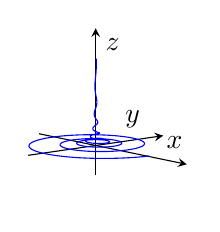
\begin{tikzpicture}[
        baseline,
        declare function = {
            solx(\a,\b,\c,\x) = \b*exp(-0.1*\x)*cos(deg(\x)) + \c*exp(-0.1*\x)*sin(deg(\x));
            soly(\a,\b,\c,\x) = -\b*exp(-0.1*\x)*sin(deg(\x)) + \c*exp(-0.1*\x)*cos(deg(\x));
            solz(\a,\b,\c,\x) = \a*exp(0.1*\x);
        }
    ]
        \begin{axis}[
            scale=0.6, % scale
            view = {50}{10},
            xmin=-1.48,xmax=2.38,ymin=-1.48,ymax=1.48, zmin = -0.5, zmax = 2.0, % range of plot
            % legend style={at={(axis cs: 1,0)}, anchor=south east}, % position of legends
            unit vector ratio = {1, 1, 1}, % aspect ratio
            axis lines = middle, % middle or box
            %axis x line = bottom, % top, middle, bottom, none: axis x line* = ... removes arrow heads
            %axis y line = left, % left, center, right, none: axis y line* = ... removes arrow heads
            xlabel = {$x$}, ylabel = {$y$}, zlabel={$z$}, % axis labels 
            xtick = {100}, ytick = {100}, ztick = {100},
        ]
            \addplot3[color=blue, variable=\t, domain=0:50, samples=1000, samples y=0]({solx(0.01, 1.4, 0.0, t)}, {soly(0.01, 1.4, 0.0, t)}, {solz(0.01, 1.4, 0.0, t)});
        \end{axis}
    \end{tikzpicture}
\end{document}